%% LaTeX-Beamer template for KIT design
%% by Erik Burger, Christian Hammer
%% title picture by Klaus Krogmann
%%
%% version 2.1
%%
%% mostly compatible to KIT corporate design v2.0
%% http://intranet.kit.edu/gestaltungsrichtlinien.php
%%
%% Problems, bugs and comments to
%% burger@kit.edu

\documentclass[18pt]{beamer}

%% SLIDE FORMAT

% use 'beamerthemekit' for standard 4:3 ratio
% for widescreen slides (16:9), use 'beamerthemekitwide'

\usepackage{templates/beamerthemekit}
%\usepackage{templates/beamerthemekitwide}
\usepackage{multirow}
%% TITLE PICTURE

% if a custom picture is to be used on the title page, copy it into the 'logos'
% directory, in the line below, replace 'mypicture' with the 
% filename (without extension) and uncomment the following line
% (picture proportions: 63 : 20 for standard, 169 : 40 for wide
% *.eps format if you use latex+dvips+ps2pdf, 
% *.jpg/*.png/*.pdf if you use pdflatex)

%\titleimage{mypicture}

%% TITLE LOGO

% for a custom logo on the front page, copy your file into the 'logos'
% directory, insert the filename in the line below and uncomment it

%\titlelogo{mylogo}

% (*.eps format if you use latex+dvips+ps2pdf,
% *.jpg/*.png/*.pdf if you use pdflatex)

%% TikZ INTEGRATION

% use these packages for PCM symbols and UML classes
% \usepackage{templates/tikzkit}
% \usepackage{templates/tikzuml}

% the presentation starts here

\title[Funkbasierte Bereichsortung]{Zuverlässige funkbasierte
Bereichsortung im Tunnelbau}
\subtitle{Masterarbeit von Marius Wodtke}
\author{Marius Wodtke}

\institute{Instuitut für angewandte Informatik und Formale Beschreibungsverfahren}

% Bibliography

\usepackage[citestyle=authoryear,bibstyle=numeric,hyperref,backend=biber]{biblatex}
\addbibresource{templates/example.bib}
\bibhang1em

\begin{document}

% change the following line to "ngerman" for German style date and logos
\selectlanguage{ngerman}

%title page
\begin{frame}
\titlepage
\end{frame}

%table of contents
\begin{frame}{Gliederung}
	\tableofcontents
\end{frame}

\section{Motivation}
\begin{frame}{Bisherige Situation}
	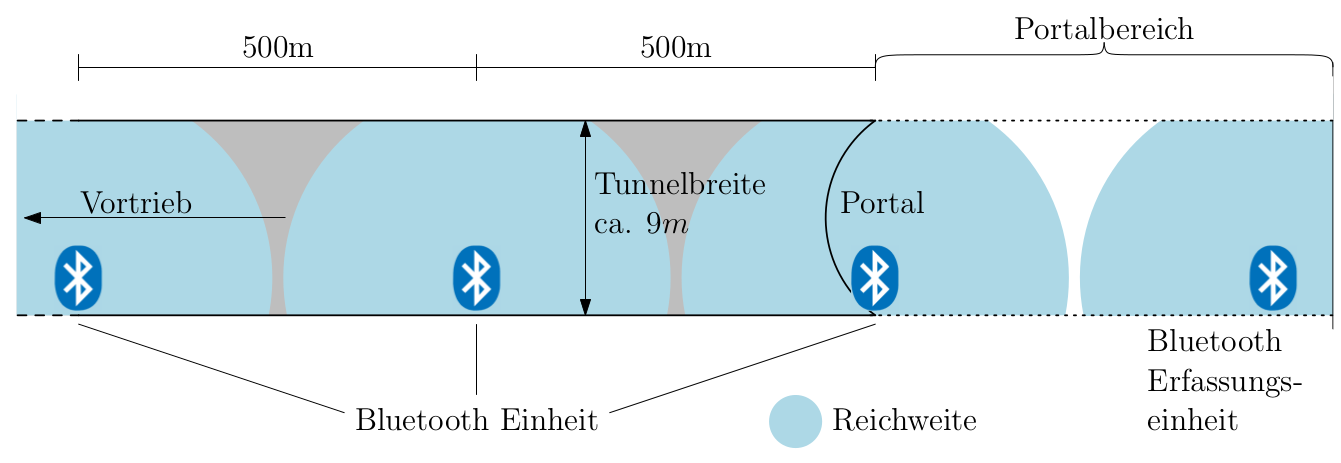
\includegraphics[width=\textwidth]{images/bisherige.png}\\
	\cite{maurer2016unterstuetzung}
\end{frame}

\begin{frame}{Zukünftige Situation}
	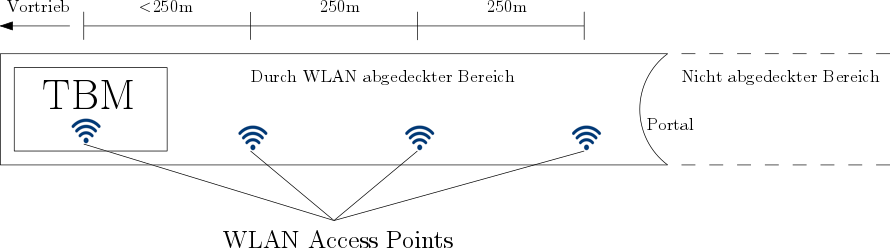
\includegraphics[width=\textwidth]{images/zukuenftige.png}
\end{frame}

\begin{frame}{Aufgabe}
	\begin{block}{Zielsetzung}
		\begin{itemize}
			\item Funkbasiertes Ortungssystem
			\item Bereichsortung (250m Abschnitte)
		\end{itemize}
	\end{block}


	\begin{block}{Anforderungen}
		\begin{itemize}
			\item Nichtintrusiv 
			\item Zuverlässige Erkennung von Abschnittswechseln
			\item Wenig Interaktion mit mobiler Einheit
		\end{itemize}
	\end{block}
\end{frame}

\section{Analyse}
\begin{frame}{Topologien}
	\begin{tabular}{c|c|c}
		\includegraphics[width=0.3\textwidth]{images/direkteselbst.eps} & \includegraphics[width=0.3\textwidth]{images/direktefern.eps} & \includegraphics[width=0.2\textwidth]{images/ohnebasis.eps}\\
		\hline
		\includegraphics[width=0.3\textwidth]{images/indirekteselbst.eps} & \includegraphics[width=0.3\textwidth]{images/indirektefern.eps} & \includegraphics[width=0.3\textwidth]{images/hybrid.eps} \\
	\end{tabular}
\end{frame}

\begin{frame}
	\begin{block}{Messgrößen}
		\begin{itemize}
			\item Time of Arrival
			\item Time Difference of Arrival
			\item Roundtrip Time of Flight
			\item Received Signal Strength (Indicator)
		\end{itemize}
	\end{block}  
	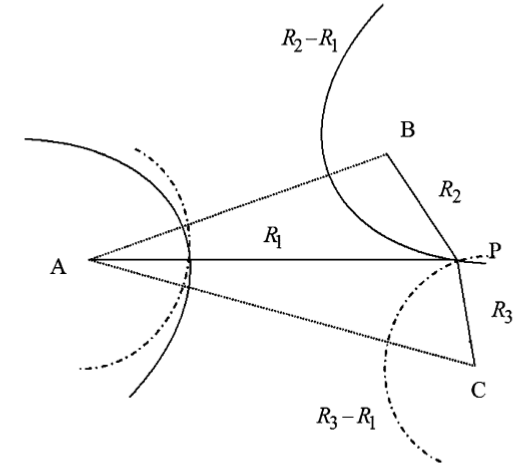
\includegraphics[width=0.3\textwidth]{images/tdoa.png} \\


	\begin{block}{Protokolle}
		\begin{itemize}
			\item 802.11
			\item Zuverlässige Erkennung von Abschnittswechseln
			\item Wenig Interaktion mit mobiler Einheit
		\end{itemize}
	\end{block} 
\end{frame}

\begin{frame}{Hardware}
	\begin{tabular}{cc}
		\multicolumn{2}{c}{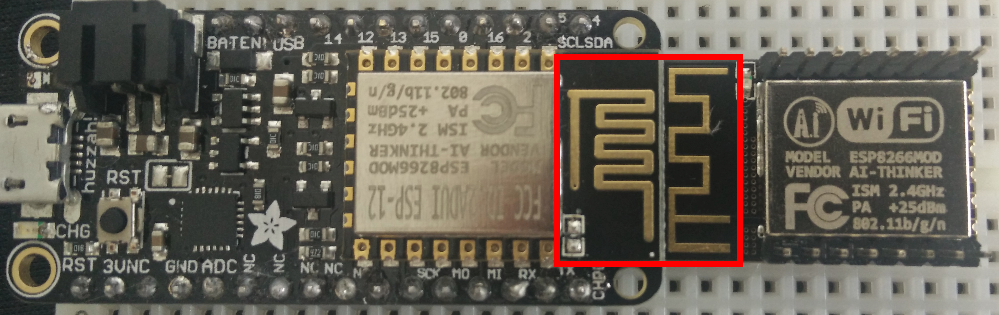
\includegraphics[width=0.9\textwidth]{images/espmodules.png}}\\
		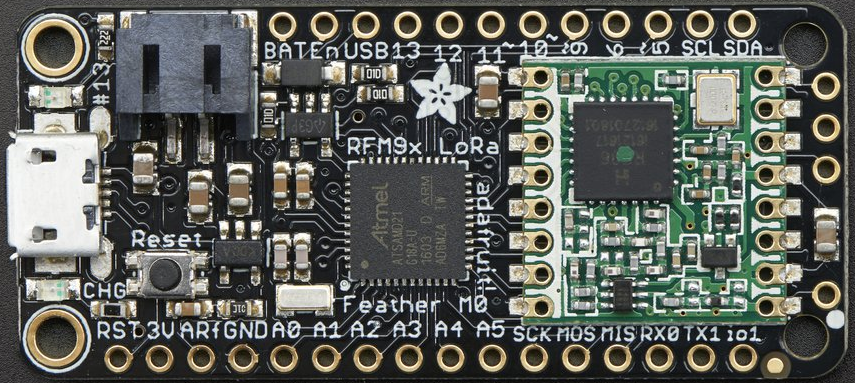
\includegraphics[width=0.45\textwidth]{images/loraada.png} & 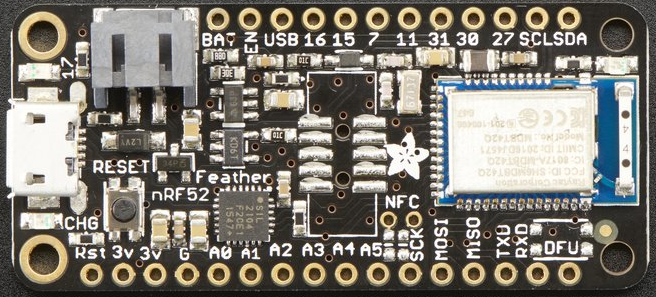
\includegraphics[width=0.45\textwidth]{images/nrf52ada.png}\\
	\end{tabular}
\end{frame}

\section{Reichweiten}
\begin{frame}{Reichweiten}
	\begin{tabular}{cc}
		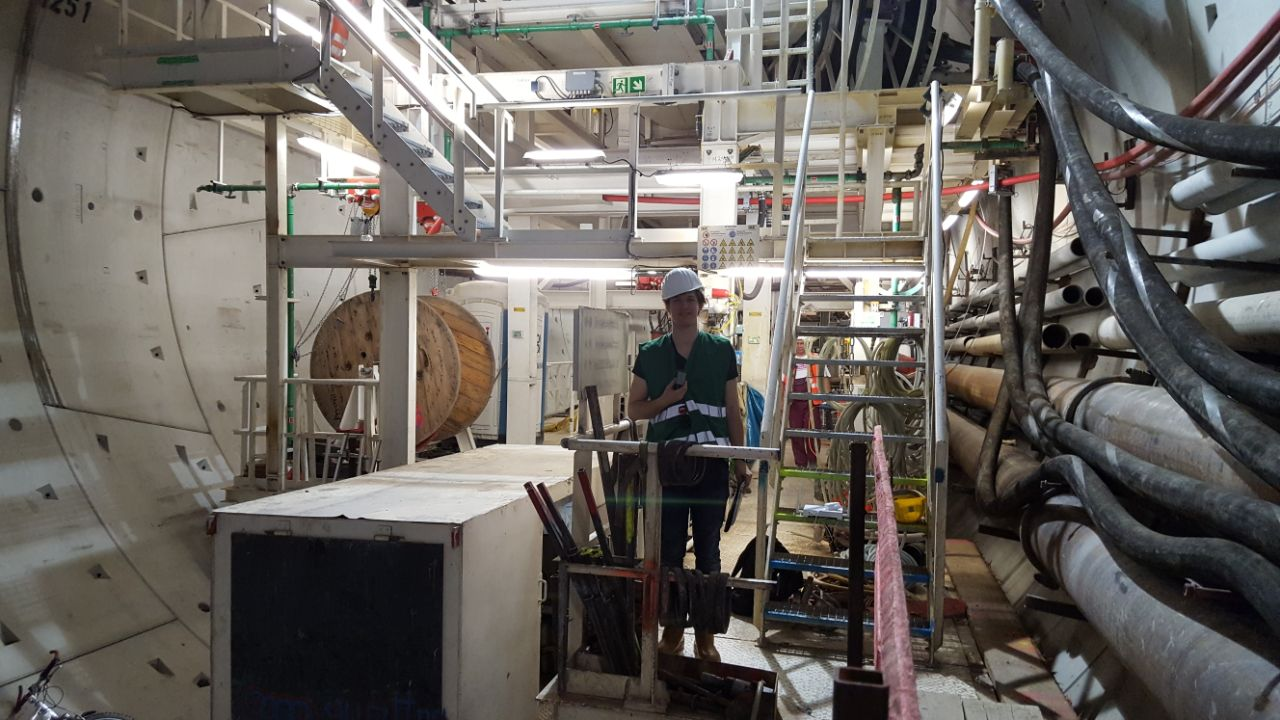
\includegraphics[width=0.45\textwidth]{images/tunnel.jpg} & 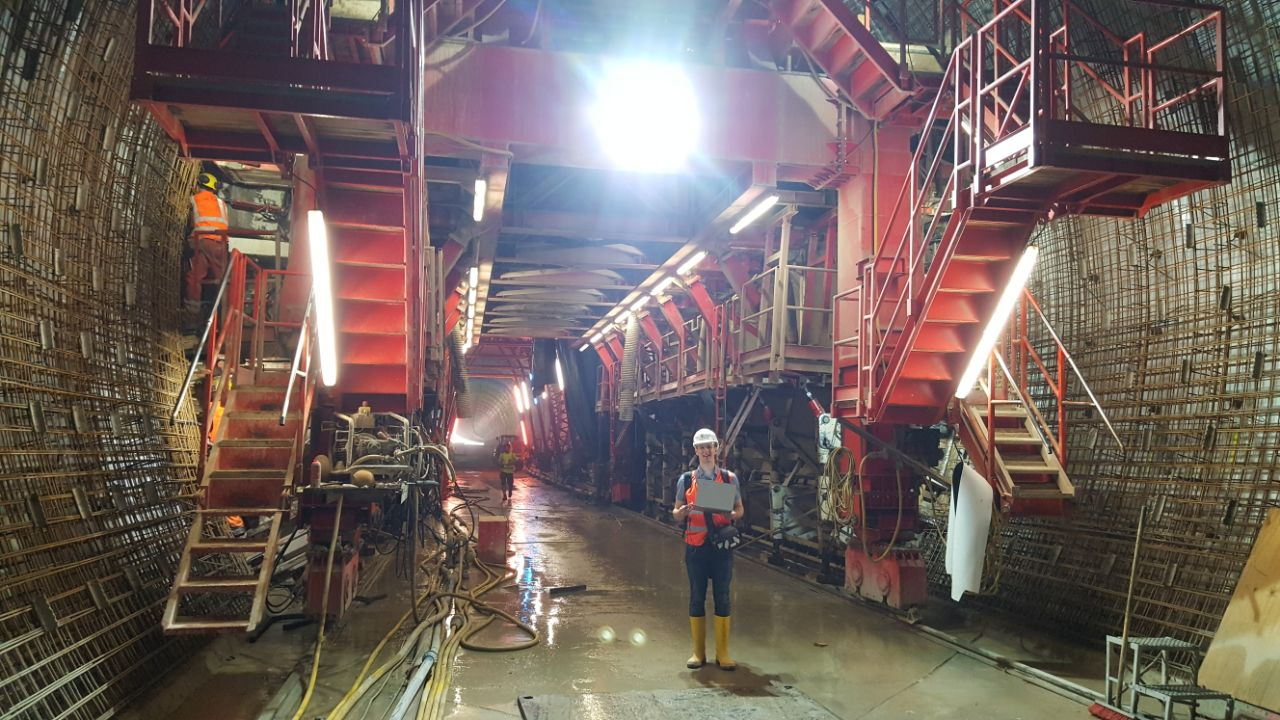
\includegraphics[width=0.45\textwidth]{images/schalungswagen.jpg}\\
		\includegraphics[width=0.45\textwidth]{images/rangewlan.eps} & \includegraphics[width=0.45\textwidth]{images/rangeblue.eps} \\
		\multicolumn{2}{c}{\includegraphics[width=0.9\textwidth]{images/rangelora.eps}}\\
	\end{tabular}
\end{frame}

\begin{frame}{Reichweiten}
	\centering
	\begin{tabular}{l|l|l}
		Protokoll & Strecke & Reichweite \\
		\hline
		BLE & Wenige Hindernisse & 32m \\
		802.11b & Wenige Hindernisse & 88m \\
		LoRa 5 dBm & Wenige Hindernisse & 250m \\
		LoRa 23 dBm & Wenige Hindernisse & 1250m \\
		\hline
		BLE & Viele Hindernisse & 14m \\
		802.11b & Viele Hindernisse & 32m \\
		LoRa 5 dBm & Viele Hindernisse & 100m \\
		LoRa 23 dBm & Viele Hindernisse & $>$350m \\
	\end{tabular}\\
\end{frame}

\section{Implementierungen}
\subsection{RADAR}
\begin{frame}{RADAR}
	\begin{tabular}{cc}
		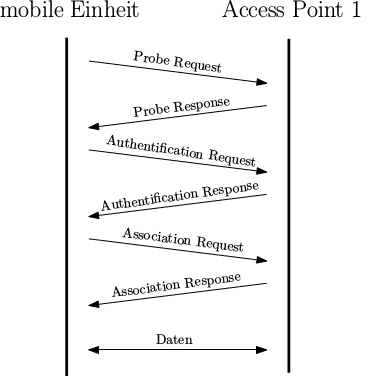
\includegraphics[height=0.5\textheight]{images/reupper.png} & 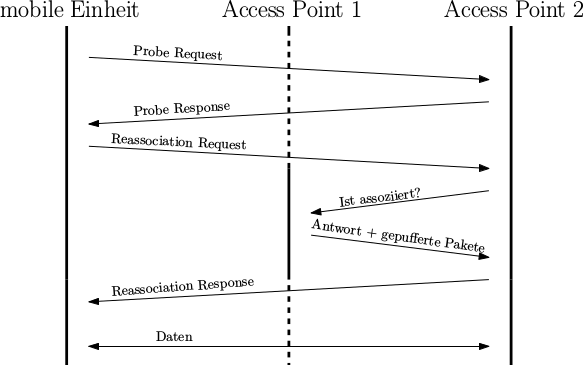
\includegraphics[height=0.5\textheight]{images/relower.png}\\
	\end{tabular}
\end{frame}

\begin{frame}
	\begin{minipage}[c][\textheight][c]{\textwidth}
		\centering
		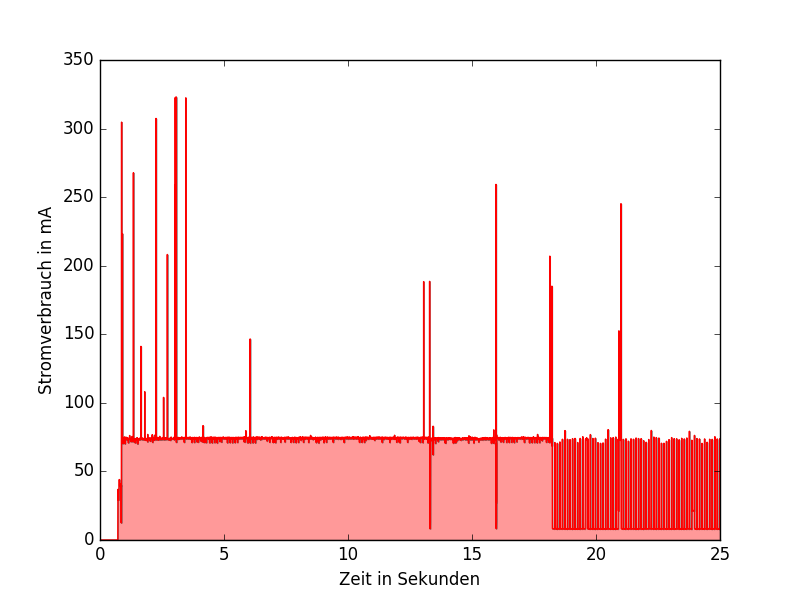
\includegraphics[height=0.95\textheight]{plots/radar5s.png}
	\end{minipage}
\end{frame}

\begin{frame}
	\begin{minipage}[c][\textheight][c]{\textwidth}
		\centering
		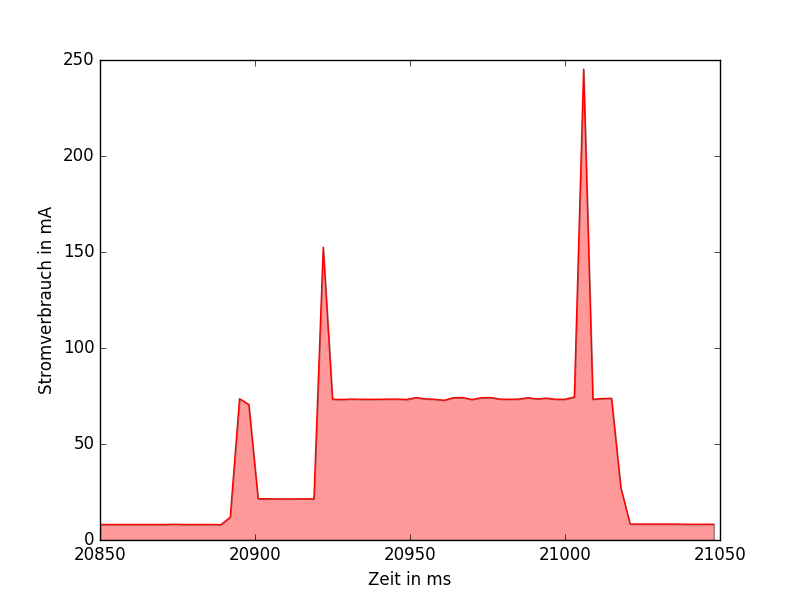
\includegraphics[height=0.95\textheight]{plots/radar5ssend.png}
	\end{minipage}
\end{frame}

\begin{frame}{WiFi-LLS}
	\begin{minipage}[c][\textheight][c]{\textwidth}
		\centering
		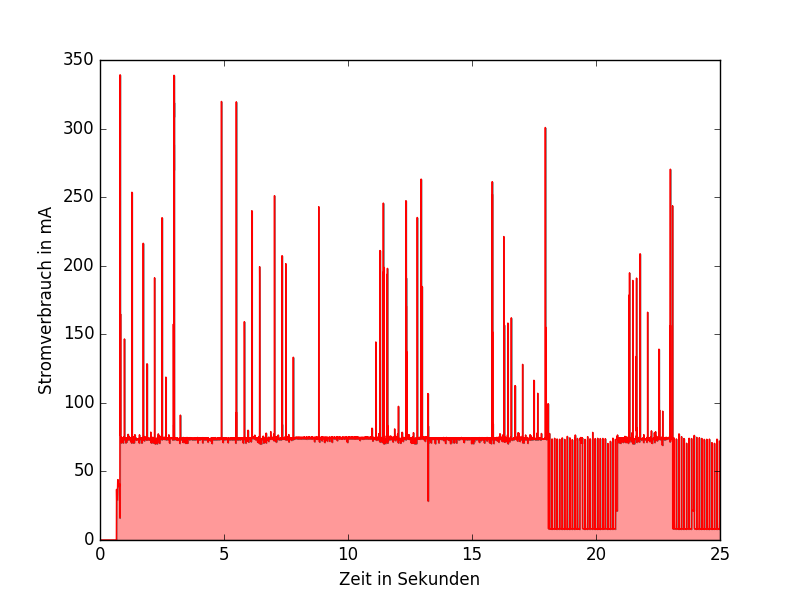
\includegraphics[height=0.95\textheight]{plots/wifills.png}
	\end{minipage}
\end{frame}

\begin{frame}
	\begin{minipage}[c][\textheight][c]{\textwidth}
		\centering
		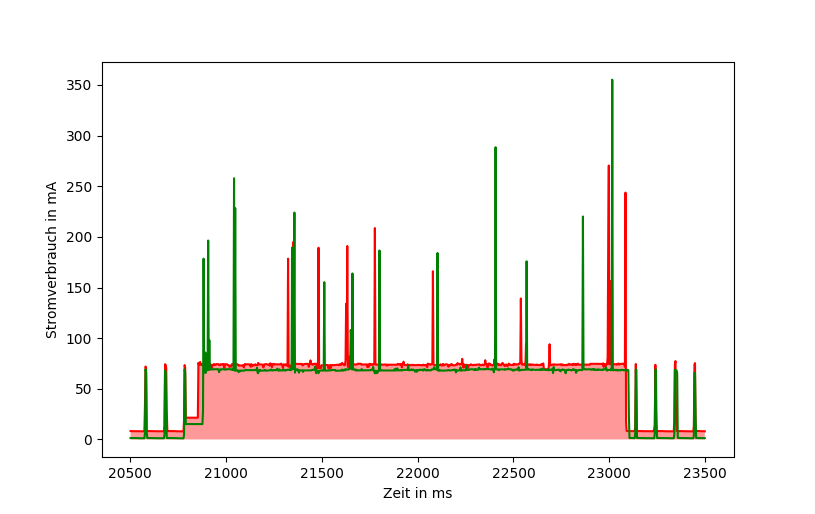
\includegraphics[height=0.95\textheight]{plots/wifillssendv.png}
	\end{minipage}
\end{frame}
%TODO Folien mergen
\begin{frame}
	\begin{minipage}[c][\textheight][c]{\textwidth}
		\centering
		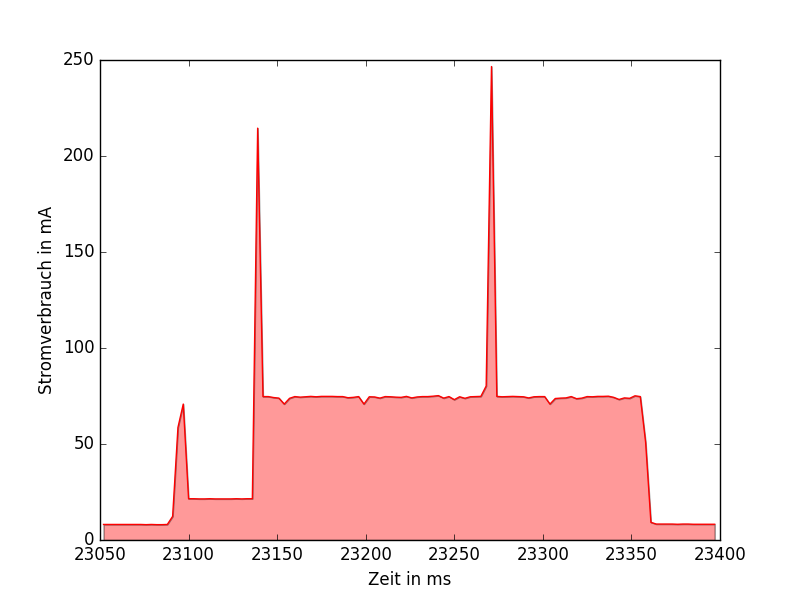
\includegraphics[height=0.95\textheight]{plots/wifills1chsend.png}
	\end{minipage}
\end{frame}

\begin{frame}{Assoziations-Lokalisierung}
	\begin{tabular}{cc}
		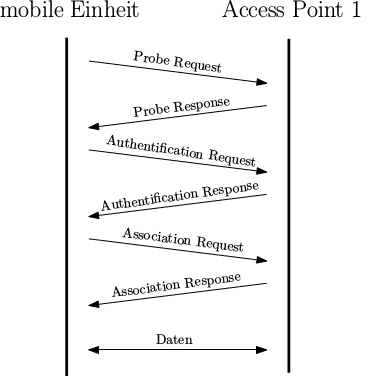
\includegraphics[height=0.5\textheight]{images/reupper.png} & 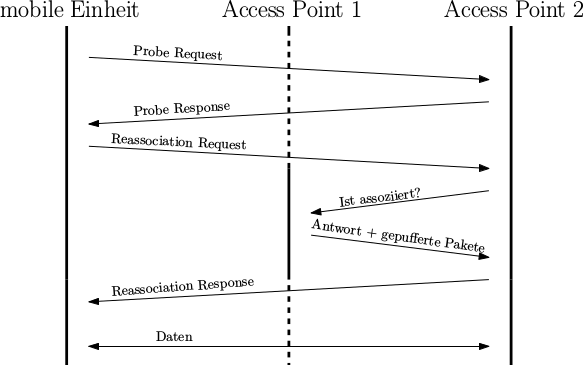
\includegraphics[height=0.5\textheight]{images/relower.png}\\
	\end{tabular}
\end{frame}

\begin{frame}
	\begin{minipage}[c][\textheight][c]{\textwidth}
		\centering
		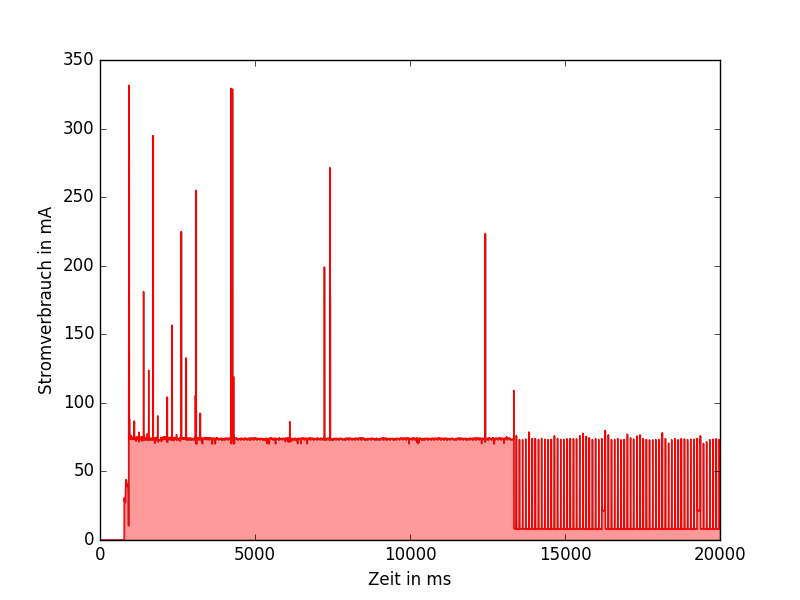
\includegraphics[height=0.95\textheight]{plots/tcphold.png}
	\end{minipage}
\end{frame}

\begin{frame}
	\begin{minipage}[c][\textheight][c]{\textwidth}
		\centering
		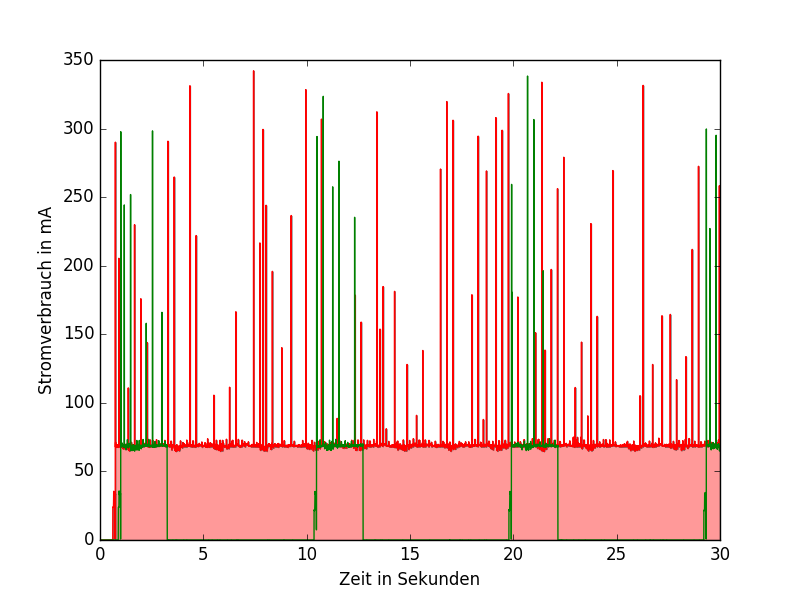
\includegraphics[height=0.95\textheight]{plots/noap.png}
	\end{minipage}
\end{frame}

\begin{frame}{Probe-Request-Lokalisierung}
	\begin{minipage}[c][\textheight][c]{\textwidth}
		\centering
		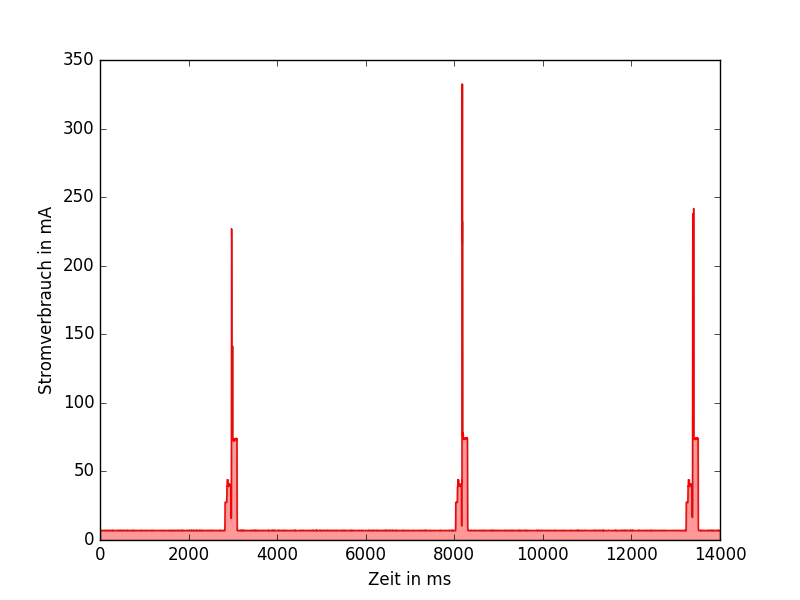
\includegraphics[height=0.95\textheight]{plots/probereqfull.png}
	\end{minipage}
\end{frame}

\begin{frame}
	\begin{minipage}[c][\textheight][c]{\textwidth}
		\centering
		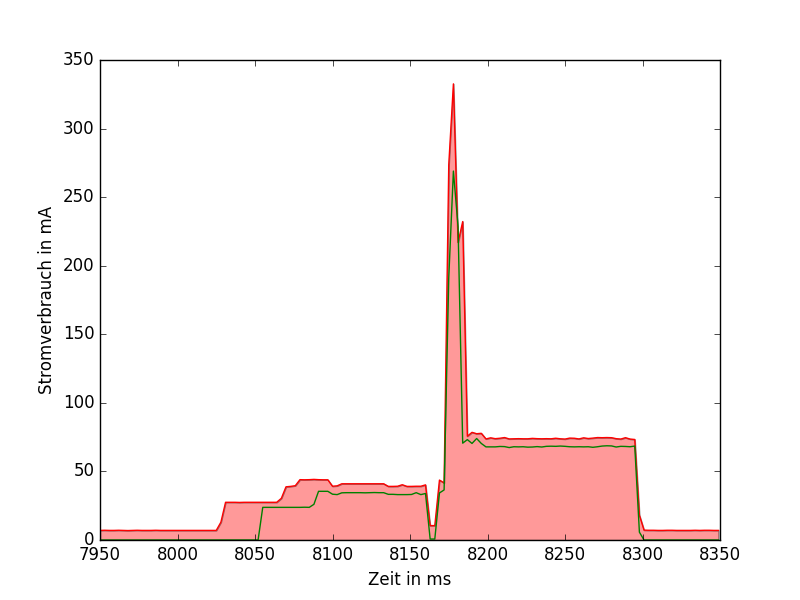
\includegraphics[height=0.95\textheight]{plots/probereqv.png}
	\end{minipage}
\end{frame}

\begin{frame}{BLE-Advertising}
	\begin{minipage}[c][\textheight][c]{\textwidth}
		\centering
		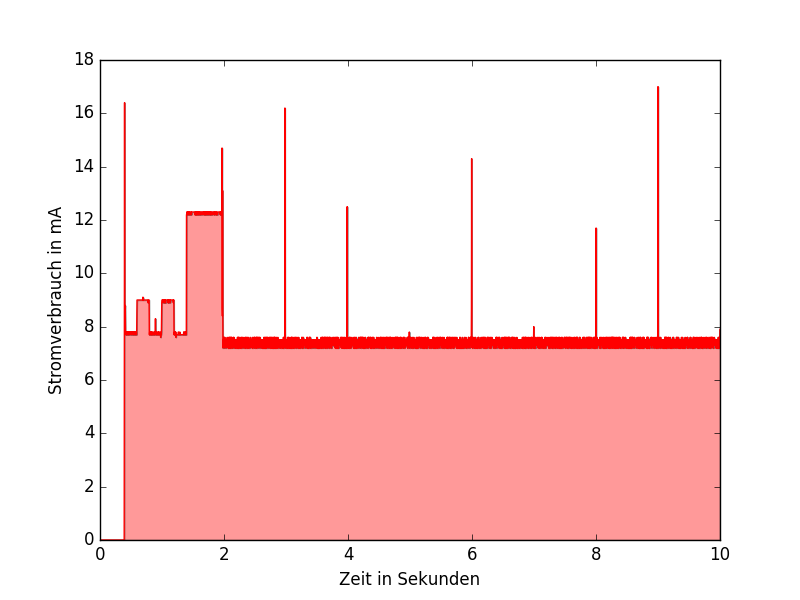
\includegraphics[height=0.95\textheight]{plots/blue.png}
	\end{minipage}
\end{frame}

\begin{frame}{LoRa}
	\begin{minipage}[c][\textheight][c]{\textwidth}
		\centering
		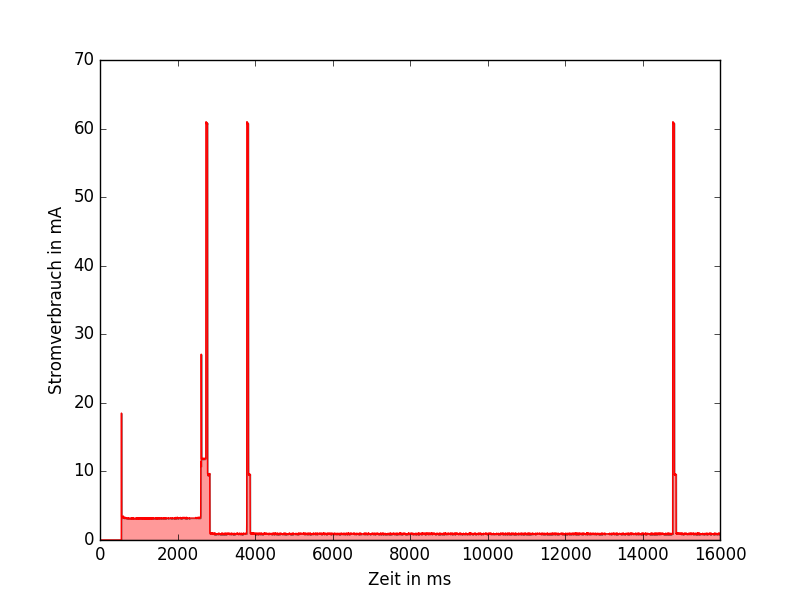
\includegraphics[height=0.95\textheight]{plots/lora5.png}
	\end{minipage}
\end{frame}

\begin{frame}
	\begin{minipage}[c][\textheight][c]{\textwidth}
		\centering
		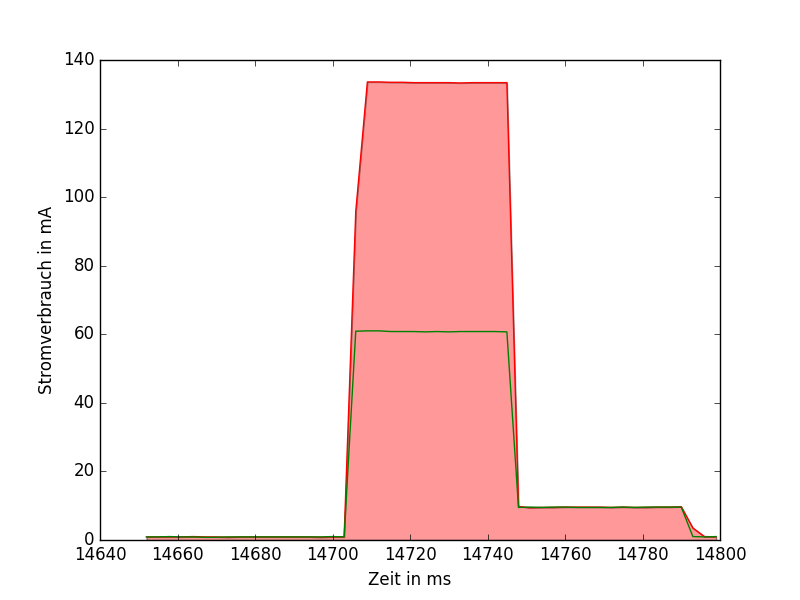
\includegraphics[height=0.95\textheight]{plots/lora235send.png}
	\end{minipage}
\end{frame}

\appendix
\beginbackup

\begin{frame}[allowframebreaks]{References}
\printbibliography
\end{frame}

\backupend

\end{document}
